% !TeX root = enterprise-architecture-digital-blueprint.tex
% !TeX encoding = UTF-8
\chapter{Arsitektur Teknologi Target dan Kesiapan AI}

\section*{Tujuan Pembelajaran}
\begin{itemize}
  \item Merumuskan arah teknologi target tingkat tinggi beserta standar teknologi organisasi.
  \item Mendokumentasikan keputusan arsitektur penting sebagai ADR (\textit{Architecture Decision Record}) lengkap dengan \textit{tradeoff}-nya.
  \item Menilai kesiapan organisasi memanfaatkan AI (\textit{Artificial Intelligence}) dari sisi kapabilitas, data, dan tata kelola.
\end{itemize}

\section{Pendahuluan}

Di banyak organisasi, keputusan teknologi diambil per proyek. Proyek
pendaftaran daring memilih satu basis data karena vendornya terbiasa
dengannya. Proyek laporan keuangan memilih alat lain karena konsultannya
menawarkan paket. Setiap pilihan masuk akal pada saat diambil. Lima tahun
kemudian, organisasi memakai empat merek basis data, enam alat pelaporan, dan
dua cara menyimpan cadangan, dan tidak ada yang dapat menjelaskan alasan tiap
pilihan. Biayanya muncul di tiga tempat: lisensi yang tumpang tindih,
keahlian yang tersebar tipis, dan celah keamanan pada teknologi yang sudah
tidak didukung vendor.

Bab 8 menetapkan bisnis target, dan Bab 9 menetapkan data dan aplikasi
target. Bab ini menutup rancangan kondisi target dengan domain teknologi.
Pertanyaannya empat: layanan teknologi apa yang dibutuhkan aplikasi target, di
mana layanan itu dijalankan, standar apa yang mengikat proyek berikutnya, dan
bagaimana keputusan besar dicatat agar dapat diperiksa kemudian. Bab ini juga
membahas AI, karena AI kini muncul di hampir setiap usulan proyek dan
menuntut kesiapan bisnis, data, aplikasi, dan tata kelola sekaligus.

Rujukan utama bab ini adalah fase D dalam ADM (\textit{Architecture
Development Method}) milik TOGAF (\textit{The Open Group Architecture
Framework}) \cite{togaf10}, lapisan teknologi ArchiMate \cite{archimate32},
format catatan keputusan dari Nygard \cite{c10-nygard2011} serta Tyree dan
Akerman \cite{c10-tyree2005}, tahap kematangan AI dan model operasi TI
(Teknologi Informasi) dari MIT CISR (\textit{Massachusetts Institute of
Technology Center for Information Systems Research})
\cite{c10-weill2024,thorogood2025}, serta survei agen AI dari SAP LeanIX
\cite{leanix2026}. Strategi migrasi dan operasi \textit{cloud} dibahas rinci di
IT40713, sedangkan kendali keamanan dan tata kelola AI dibahas rinci di
IT40813.

\IfFileExists{../figures/ch10-diagram-konsep.png}{%

Gambar \ref{fig:ch10-ilustrasi-bab} merangkum hubungan komponen dan konsep utama bab ini.
\begin{figure}[!htb]
  \centering
  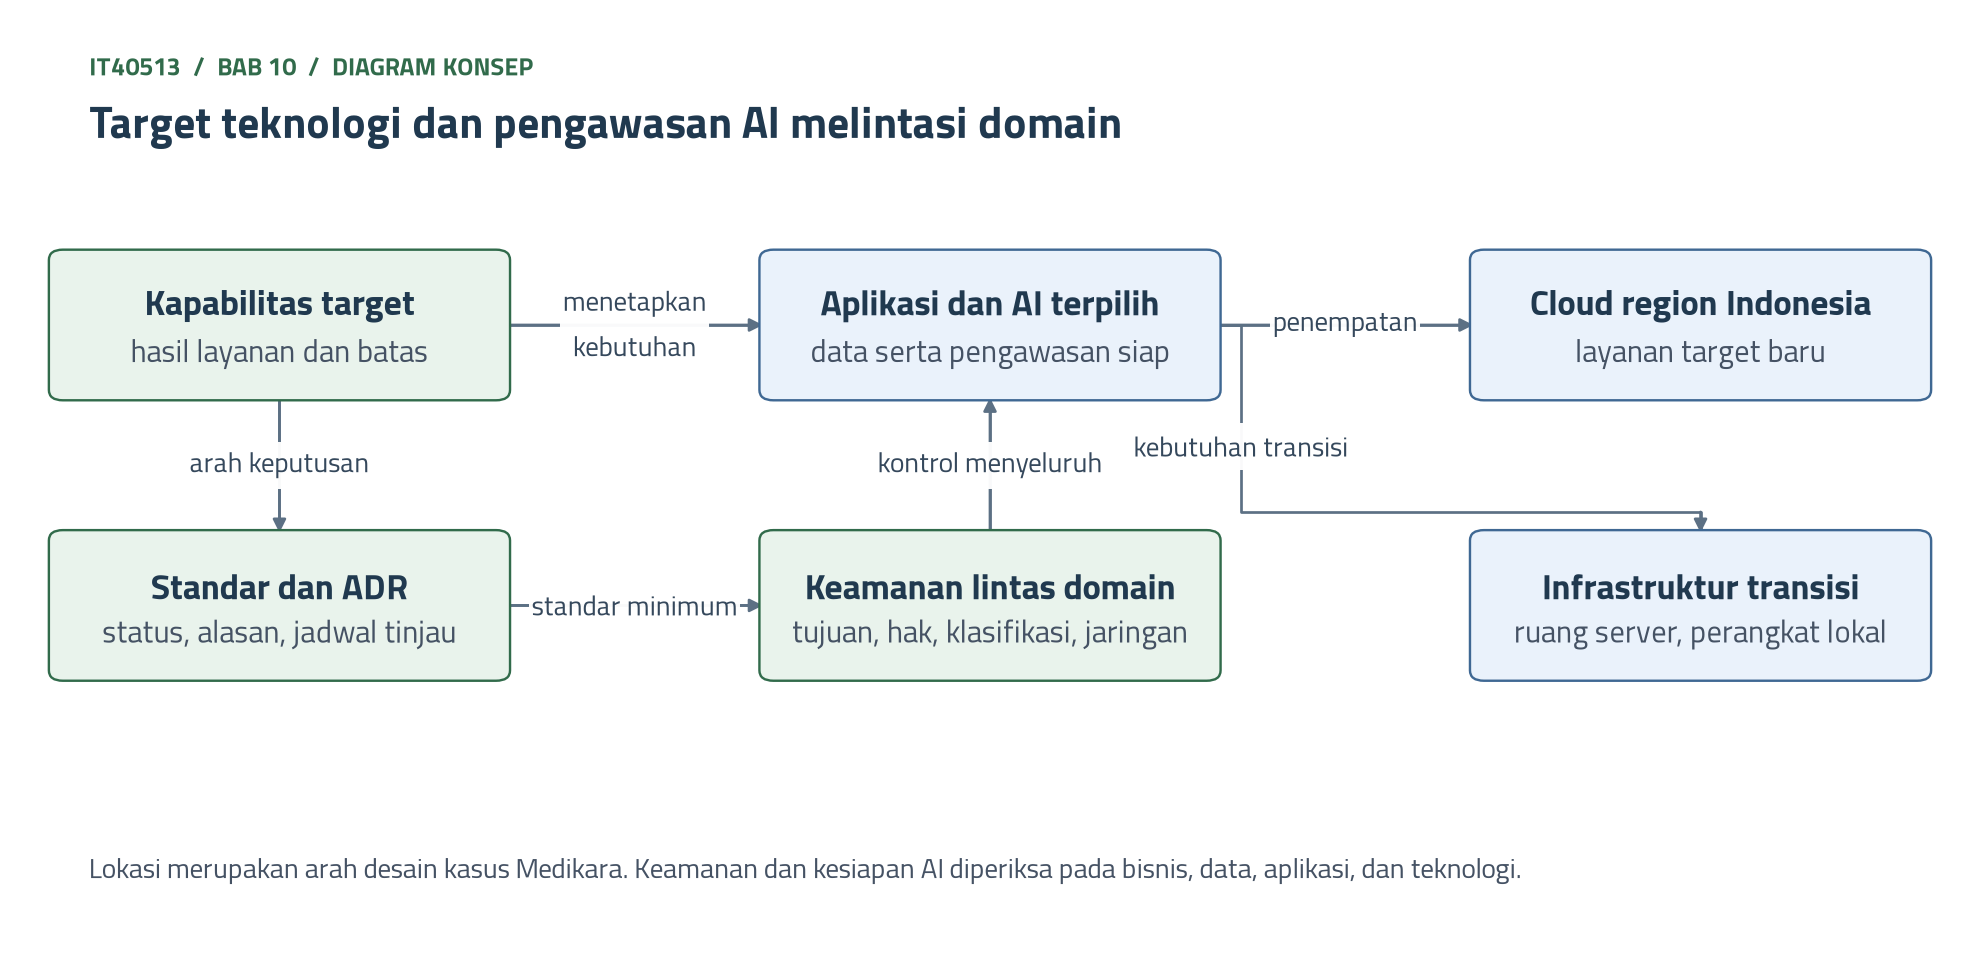
\includegraphics[width=\textwidth]{../figures/ch10-diagram-konsep.png}
  \caption{Target teknologi dan pengawasan AI melintasi domain}
  \label{fig:ch10-ilustrasi-bab}
\end{figure}
}{}

\section{Arsitektur Teknologi Tingkat Tinggi}

Arsitektur teknologi menjelaskan layanan teknologi yang dibutuhkan aplikasi
dan data target, beserta tempat layanan itu dijalankan. Dalam ADM, pekerjaan
ini berada di fase D. Langkahnya sama dengan fase B dan C: memilih model
rujukan dan \textit{viewpoint}, memotret kondisi saat ini, merancang kondisi
target, mencatat selisihnya, lalu menurunkan selisih itu menjadi calon
komponen peta jalan \cite{togaf10}. Kondisi saat ini sudah dipotret di Bab 7,
sehingga bab ini berfokus pada kondisi target. Dalam ArchiMate, unsur yang
dipakai antara lain \textit{technology service}, \textit{node},
\textit{system software}, dan \textit{communication network}
\cite{archimate32}.

Kata kuncinya adalah tingkat tinggi. Arsitektur teknologi di tingkat
\textit{enterprise} tidak memilih ukuran server atau versi pustaka
perangkat lunak. Yang diputuskan adalah arah: layanan teknologi bersama apa
yang disediakan untuk seluruh organisasi, lokasi mana yang menjadi tempat
utama, dan aturan apa yang dipakai ketika sebuah proyek memilih teknologi.
Rincian di bawah arah itu menjadi urusan arsitektur solusi tiap proyek.

Analoginya seperti merancang utilitas sebuah gedung perkantoran. Penyewa
tidak perlu tahu merek trafo atau letak pipa. Yang dibutuhkan penyewa adalah
jaminan listrik, air, lift, dan pengamanan pintu yang sama di setiap lantai.
Pengelola gedung memutuskan kapasitas, jalur, dan standar perlengkapannya
sekali untuk seluruh gedung. Bila tiap penyewa memasang genset dan pompa
sendiri, gedung tetap berjalan, tetapi biaya dan risikonya berlipat.

Gambar \ref{fig:ch10-arah-teknologi} memperlihatkan tiga lapis pertanyaan itu
untuk Medikara. Lapis atas berisi aplikasi target dari Bab 9. Lapis tengah
berisi layanan teknologi bersama yang dibutuhkan aplikasi tersebut. Lapis
bawah berisi lokasi tempat layanan itu dijalankan.

\begin{figure}[!htb]
  \centering
  \begin{tikzpicture}[
  font=\scriptsize,
  kotak/.style={draw, rounded corners, minimum height=0.85cm, text width=1.6cm,
                align=center, font=\scriptsize},
  lokasi/.style={draw, rounded corners, minimum height=0.85cm, text width=2.6cm,
                 align=center, font=\scriptsize},
  pita/.style={draw, rounded corners, fill=praditagreen!15, minimum height=1.2cm,
               text width=1.6cm, align=center, font=\scriptsize\bfseries},
  panah/.style={-{Stealth[length=2mm]}, thick}
]
  % Pita kiri: tiga lapis pertanyaan arsitektur teknologi.
  \node[pita] (p1) at (0,3.4) {Aplikasi\\target};
  \node[pita] (p2) at (0,1.7) {Layanan\\teknologi};
  \node[pita] (p3) at (0,0) {Lokasi\\penerapan};

  % Lapis atas: aplikasi target dari Bab 9.
  \node[kotak, fill=blue!8] at (2.2,3.4) {SIMRS\\terpadu};
  \node[kotak, fill=blue!8] at (4.15,3.4) {MPI};
  \node[kotak, fill=blue!8] at (6.1,3.4) {Platform\\integrasi};
  \node[kotak, fill=blue!8] at (8.05,3.4) {Medikara+,\\portal mitra};
  \node[kotak, fill=blue!8] at (10.0,3.4) {ERP dan\\platform data};

  % Lapis tengah: layanan teknologi yang dirumuskan di fase D.
  \node[kotak, fill=orange!12] at (2.2,1.7) {Basis data\\terkelola};
  \node[kotak, fill=orange!12] at (4.15,1.7) {Identitas\\terpusat};
  \node[kotak, fill=orange!12] at (6.1,1.7) {Integrasi dan\\\textit{API gateway}};
  \node[kotak, fill=orange!12] at (8.05,1.7) {Penyim\-panan,\\cadangan};
  \node[kotak, fill=orange!12] at (10.0,1.7) {Pemantauan,\\catatan akses};

  % Lapis bawah: lokasi penerapan.
  \node[lokasi, fill=green!10] at (3.0,0) {\textit{Cloud} publik region\\Indonesia {\tiny\mdseries(arah utama)}};
  \node[lokasi, fill=blue!8] at (6.1,0) {Ruang server rumah sakit\\{\tiny\mdseries(selama transisi)}};
  \node[lokasi, fill=blue!8] at (9.2,0) {Rumah sakit dan klinik\\{\tiny\mdseries(jaringan, perangkat lokal)}};

  \draw[panah] (p1.south) -- (p2.north);
  \draw[panah] (p2.south) -- (p3.north);
  \node[font=\tiny, gray, anchor=west] at (0.1,2.55) {membutuhkan};
  \node[font=\tiny, gray, anchor=west] at (0.1,0.85) {dijalankan di};
\end{tikzpicture}

  \caption{Arah teknologi target Medikara: aplikasi target membutuhkan layanan
           teknologi bersama, dan layanan itu dijalankan di lokasi yang
           ditetapkan}
  \label{fig:ch10-arah-teknologi}
\end{figure}

Dua contoh memperlihatkan nilai layanan teknologi bersama:

\begin{enumerate}
  \item Kelima aplikasi target pada Gambar \ref{fig:ch10-arah-teknologi}
        membutuhkan basis data. Bila tiap proyek memilih sendiri, lima tim
        memelihara lima jenis basis data dengan lima cara pencadangan. Bila
        organisasi menyediakan satu layanan basis data terkelola dengan dua
        pilihan standar, pemeliharaan, pencadangan, dan pemantauannya
        dikerjakan sekali.
  \item Peraturan Menteri Kesehatan Nomor 24 Tahun 2022 mewajibkan cadangan
        rekam medis elektronik diletakkan di tempat yang berbeda dari lokasi
        fasilitas pelayanan kesehatan \cite{permenkes24-2022}. Medikara punya
        5 rumah sakit dan 18 klinik pratama, sehingga ada 23 fasilitas yang
        terkena kewajiban itu. Tanpa layanan penyimpanan dan cadangan
        bersama, 23 fasilitas mencari jalan keluarnya sendiri-sendiri.
        Dengan layanan bersama, kewajiban itu dipenuhi sekali untuk
        seluruhnya.
\end{enumerate}

\subsection*{Pilihan lokasi penerapan}

Lokasi penerapan menjawab pertanyaan di mana layanan teknologi dijalankan.
National Institute of Standards and Technology (NIST) membedakan empat model
penerapan \textit{cloud}, yaitu \textit{private}, \textit{community},
\textit{public}, dan \textit{hybrid} \cite{nist800-145}. Ditambah
\textit{on-premise}, yaitu server milik sendiri di ruang server atau pusat data
sendiri, organisasi seperti Medikara biasanya memilih di antara empat pilihan
pada Tabel \ref{tab:ch10-lokasi}. \textit{Community cloud} jarang dipakai
swasta, sehingga tidak dimuat.

\begin{table}[!htb]
  \centering
  \caption{Empat pilihan lokasi penerapan pada tingkat keputusan arsitektur}
  \label{tab:ch10-lokasi}
  \small
  \begin{tabularx}{\textwidth}{lXXX}
    \hline
    \textbf{Pilihan} & \textbf{Artinya} & \textbf{Cocok untuk} & \textbf{Yang dikorbankan} \\
    \hline
    \textit{On-premise} & Server milik dan dikelola sendiri di lokasi sendiri &
      Sistem yang terikat perangkat lokal atau kontrak lama &
      Modal awal besar, kapasitas tetap, pemulihan bencana ditanggung sendiri \\
    \hline
    \textit{Private cloud} & Infrastruktur \textit{cloud} khusus untuk satu organisasi &
      Organisasi besar yang butuh kendali penuh dan elastisitas &
      Tetap butuh tim dan skala besar agar efisien \\
    \hline
    \textit{Public cloud} & Infrastruktur penyedia yang dipakai banyak pelanggan, dibayar sesuai pemakaian &
      Beban yang naik turun, layanan baru, analitik &
      Ketergantungan pada penyedia, biaya berulang yang harus dikendalikan \\
    \hline
    \textit{Hybrid cloud} & Dua model atau lebih yang terpisah tetapi terhubung &
      Masa transisi, beban yang belum dapat dipindahkan &
      Dua lingkungan yang harus dikelola dan diamankan sekaligus \\
    \hline
  \end{tabularx}
\end{table}

Pertanyaan kemudian muncul: siapa yang memutuskan lokasi tiap aplikasi? Di
tingkat EA (\textit{Enterprise Architecture}), yang diputuskan adalah arah dan
aturan pemilihannya, misalnya "\textit{cloud} publik di region Indonesia
untuk aplikasi baru, kecuali ada alasan tertulis". Penilaian per aplikasi
dengan strategi 7R, rancangan \textit{landing zone}, dan operasi \textit{cloud}
sehari-hari dibahas rinci di IT40713.

Untuk rekam medis, arah itu dibatasi regulasi. Pasal 20 Peraturan Menteri
Kesehatan Nomor 24 Tahun 2022 mengizinkan rekam medis elektronik disimpan di
server, di sistem komputasi awan yang tersertifikasi, atau di media digital
lain yang tersertifikasi, dan mewajibkan cadangan di tempat yang berbeda dari
lokasi fasilitas. Pasal 22 mengatur penyimpanan lewat kerja sama dengan
Penyelenggara Sistem Elektronik bagi fasilitas yang sumber dayanya terbatas.
Penyelenggara itu harus punya fasilitas penyimpanan data di dalam negeri dan
mendapat rekomendasi dari unit Kementerian Kesehatan yang membidangi data dan
informasi \cite{permenkes24-2022}.

\begin{kasus}[title={Kasus Medikara Health: Arah Modernisasi ke Cloud dan Batasannya}]
Strategi 2026 sampai 2030 memuat modernisasi ke \textit{cloud}. Tim arsitektur
menerjemahkannya menjadi tiga kalimat arah teknologi target:

\begin{enumerate}
  \item \textit{Cloud} publik di region Indonesia menjadi lokasi utama untuk
        aplikasi target baru: SIMRS (Sistem Informasi Manajemen Rumah Sakit)
        terpadu, MPI (\textit{Master Patient Index}), platform integrasi, dan
        platform data.
  \item Ruang server di tiap rumah sakit tetap dipakai selama transisi untuk SIMRS
        lama yang belum dipindahkan, lalu ditutup bertahap setelah konsolidasi.
  \item Rumah sakit dan klinik hanya menyimpan perangkat yang memang harus
        dekat dengan pasien, misalnya perangkat medis yang tersambung dan
        jaringan lokal.
\end{enumerate}

Arah itu punya empat batasan. Pertama, regulasi rekam medis yang dibahas di
atas. Kedua, jaringan. Misalkan dua klinik di pinggiran Bogor hanya punya satu
jalur internet. Bila jalur itu putus setelah pendaftaran pindah ke SIMRS
pusat, pendaftaran di klinik tersebut berhenti. Jalur cadangan harus ada
lebih dahulu. Ketiga, keterampilan. Tim TI Medikara terbiasa merawat server
fisik, belum terbiasa mengelola biaya dan keamanan \textit{cloud}. Keempat,
kontrak vendor SIMRS lama yang masih berjalan.

Kalimat arah ini belum memutuskan lokasi penyimpanan rekam medis. Keputusan
itu cukup besar untuk dicatat tersendiri sebagai ADR-001, yang dibahas pada
seksi tentang ADR.
\end{kasus}

\section{Standar Teknologi dan Technology Reference Model}

Misalkan katalog teknologi yang disusun di Bab 7 mencatat empat merek basis
data, tiga keluarga sistem operasi server, dua alat cadangan, dan enam alat
pelaporan di Medikara. Tidak satu pun dipilih dengan buruk. Masalahnya, tidak
ada daftar yang menyatakan teknologi mana yang boleh dipakai proyek
berikutnya. Akibatnya, setiap proyek baru mengulang perdebatan yang sama, dan
setiap vendor baru membawa teknologinya sendiri.

Katalog standar teknologi menutup celah itu. Katalog ini berisi daftar
teknologi yang disepakati organisasi, lengkap dengan versinya, statusnya,
pemiliknya, dan jadwal peninjauannya. TOGAF menyebutnya \textit{Technology
Standards catalog}, salah satu artefak yang lazim dihasilkan di fase D
\cite{togaf10}. Status menjadi bagian terpenting, karena status menyatakan
apa yang boleh dilakukan proyek terhadap teknologi itu. Gambar
\ref{fig:ch10-siklus-standar} memperlihatkan siklus status yang dipakai bab
ini.

\begin{figure}[!htb]
  \centering
  \begin{tikzpicture}[
  font=\scriptsize,
  kotak/.style={draw, rounded corners, minimum height=1.05cm, text width=1.7cm,
                align=center, font=\scriptsize\bfseries},
  panah/.style={-{Stealth[length=2mm]}, thick}
]
  \node[kotak, fill=blue!8] (usul) at (0,0) {Usulan\\{\tiny\mdseries diajukan proyek}};
  \node[kotak, fill=blue!8] (baru) at (2.5,0) {Baru\\{\tiny\mdseries uji coba terbatas}};
  \node[kotak, fill=green!10] (pakai) at (5.0,0) {Dipakai\\{\tiny\mdseries wajib untuk proyek baru}};
  \node[kotak, fill=orange!12] (batas) at (7.5,0) {Dibatasi\\{\tiny\mdseries hanya dipelihara}};
  \node[kotak, fill=red!22] (henti) at (10.0,0) {Dihentikan\\{\tiny\mdseries tanggal akhir pasti}};
  \node[kotak, fill=gray!35] (tolak) at (2.5,-1.85) {Ditolak\\{\tiny\mdseries alasan dicatat}};

  \draw[panah] (usul) -- (baru);
  \draw[panah] (baru) -- (pakai);
  \draw[panah] (pakai) -- (batas);
  \draw[panah] (batas) -- (henti);
  \draw[panah] (baru) -- (tolak);

  \node[font=\tiny, gray] at (1.25,0.78) {disetujui dicoba};
  \node[font=\tiny, gray] at (3.75,0.78) {lolos uji coba};
  \node[font=\tiny, gray] at (6.25,0.78) {ada pengganti};
  \node[font=\tiny, gray] at (8.75,0.78) {migrasi selesai};
  \node[font=\tiny, gray, anchor=west] at (2.6,-0.95) {gagal uji coba};

  \node[font=\tiny, align=center, text width=6.2cm, anchor=north west]
    at (4.15,-1.3) {Setiap perpindahan status diputuskan forum arsitektur,
    dicatat sebagai ADR, dan ditinjau ulang paling lambat 12 bulan sekali.};
\end{tikzpicture}

  \caption{Siklus status standar teknologi: setiap teknologi masuk lewat uji
           coba dan keluar lewat tanggal akhir yang pasti}
  \label{fig:ch10-siklus-standar}
\end{figure}

Analoginya seperti formularium di rumah sakit, yaitu daftar obat yang
disepakati komite. Dokter meresepkan obat dari daftar itu. Obat di luar daftar
butuh persetujuan khusus beserta alasannya. Obat baru dicoba terbatas lebih
dahulu, dan obat lama dikeluarkan dari daftar ketika ada pengganti yang lebih
baik. Katalog standar teknologi bekerja dengan cara yang sama untuk server,
basis data, dan platform.

Organisasi tidak harus menyusun status dari nol. Technology Radar dari
Thoughtworks, yang terbit dua kali setahun, memakai empat cincin: Adopt,
Trial, Assess, dan Caution \cite{c10-thoughtworks-radar}. Bedanya perlu
diingat. Radar itu pendapat satu perusahaan tentang industri, sedangkan
katalog standar adalah keputusan organisasi yang mengikat proyeknya sendiri.

Tabel \ref{tab:ch10-katalog} memuat potongan katalog standar target Medikara.
Isinya sengaja ditulis sebagai kategori, bukan merek dagang, agar polanya
dapat dipakai organisasi lain.

\begin{table}[!htb]
  \centering
  \caption{Potongan katalog standar teknologi target Medikara}
  \label{tab:ch10-katalog}
  \small
  \begin{tabularx}{\textwidth}{XlX}
    \hline
    \textbf{Standar} & \textbf{Status} & \textbf{Catatan} \\
    \hline
    Basis data relasional sumber terbuka sebagai layanan terkelola & Dipakai & Pilihan pertama untuk aplikasi baru \\
    \hline
    Basis data relasional komersial bawaan SIMRS lama & Dibatasi & Hanya dipelihara sampai SIMRS diganti \\
    \hline
    Sistem operasi server versi lama tanpa dukungan vendor & Dihentikan & Tanggal akhir 31 Desember 2027 \\
    \hline
    Layanan identitas terpusat dengan autentikasi multifaktor & Dipakai & Wajib untuk semua aplikasi baru \\
    \hline
    HL7 (\textit{Health Level Seven}) FHIR (\textit{Fast Healthcare Interoperability Resources}) untuk data klinis & Dipakai & Sejalan dengan SATUSEHAT \\
    \hline
    Platform analitik dan \textit{dashboard} tunggal & Baru & Uji coba di rumah sakit Depok sampai Juni 2027 \\
    \hline
    \textit{Spreadsheet} sebagai sumber laporan manajemen & Dibatasi & Diganti platform analitik \\
    \hline
  \end{tabularx}
\end{table}

Standardisasi punya dua konsekuensi yang perlu dihitung. Pertama, biaya rutin
turun. Misalkan lisensi dan dukungan empat merek basis data menghabiskan
Rp2,4 miliar per tahun, dan konsolidasi menjadi dua merek menurunkannya
menjadi Rp1,5 miliar. Penghematannya Rp0,9 miliar per tahun. Keahlian ikut
terpusat: dengan dua administrator per merek agar ada pengganti saat cuti,
empat merek membutuhkan delapan orang, sedangkan dua merek cukup empat orang.
Kedua, ada biaya di depan dan biaya tersembunyi. Misalkan migrasi dari dua
merek yang dihentikan memakan biaya satu kali Rp2,7 miliar, sehingga
penghematan tadi baru menutup biaya migrasi dalam tiga tahun. Ketergantungan
pada vendor yang lebih sedikit juga makin besar, dan proyek yang membutuhkan
teknologi baru terhambat bila jalur status Baru tidak tersedia.

\subsection*{Technology reference model sebagai bahasa bersama}

Katalog standar menjawab pertanyaan teknologi apa yang dipakai. Pertanyaan
berikutnya: kategori apa saja yang wajib punya standar? Di sinilah
\textit{technology reference model} berguna. Model ini adalah taksonomi
layanan platform yang generik, misalnya layanan manajemen data, layanan
keamanan, layanan jaringan, dan layanan antarmuka pengguna. TOGAF
\textit{Technical Reference Model} adalah contoh yang paling dikenal. Pada
TOGAF edisi ke-10, model ini tidak lagi menjadi bagian inti standar dan
tersedia sebagai \textit{Series Guide} G175, yang oleh The Open Group sendiri
disebut konten historis dari versi sebelumnya, tetapi masih berguna
\cite{c10-togaf-trm}.

Nilai utama model rujukan ini adalah bahasa bersama. Ketika bagian keuangan
menyebut "sistem laporan", tim TI menyebut "platform analitik", dan vendor
menyebut "\textit{business intelligence}", ketiganya merujuk kategori yang
sama. Tanpa kategori bersama, katalog standar mudah bolong: kategori yang
tidak pernah dibicarakan tidak pernah punya standar.

Dua hal pada standar teknologi sering tertukar. Pembagiannya begini.
\textit{Technology reference model} adalah rak berlabel: rak basis data, rak
identitas, rak integrasi. Rak itu sama untuk banyak organisasi. Katalog
standar adalah isi rak: produk dan versi yang dipilih satu organisasi beserta
statusnya. Organisasi boleh meminjam rak dari luar, tetapi isi raknya harus
diputuskan sendiri.

\section{Keamanan sebagai Concern Lintas Domain}

Keamanan sering digambar sebagai satu lapisan tambahan di bawah atau di
samping arsitektur. Gambaran itu menyesatkan. Keputusan keamanan tersebar di
semua domain: siapa yang boleh melihat data pasien adalah keputusan bisnis,
klasifikasi data adalah keputusan data, pemeriksaan hak di dalam aplikasi
adalah keputusan aplikasi, dan pemisahan jaringan adalah keputusan teknologi.
Karena itu keamanan disebut \textit{concern} lintas domain. Tabel
\ref{tab:ch10-keamanan} memperlihatkan sebarannya.

\begin{table}[!htb]
  \centering
  \caption{Keamanan sebagai \textit{concern} yang muncul di setiap domain
           arsitektur}
  \label{tab:ch10-keamanan}
  \small
  \begin{tabularx}{\textwidth}{lXX}
    \hline
    \textbf{Domain} & \textbf{Pertanyaan keamanan} & \textbf{Contoh keputusan arsitektur} \\
    \hline
    Bisnis & Peran apa yang boleh melihat rekam medis? & Hanya tenaga kesehatan yang merawat pasien itu \\
    \hline
    Data & Data mana yang paling dilindungi? & Data kesehatan diklasifikasi sebagai data pribadi spesifik \\
    \hline
    Aplikasi & Di mana hak akses diperiksa? & Semua aplikasi memakai satu layanan identitas dan peran baku \\
    \hline
    Teknologi & Dari mana basis data klinis dapat dijangkau? & Hanya dari zona aplikasi, tidak dari jaringan umum \\
    \hline
  \end{tabularx}
\end{table}

Baris data pada tabel tersebut bukan pilihan bebas. Undang-Undang (UU) Nomor 27
Tahun 2022 tentang Pelindungan Data Pribadi (PDP) menggolongkan data dan
informasi kesehatan sebagai data pribadi yang bersifat spesifik
\cite{uu27-2022-pdp}. Kewajiban yang menyertainya dibahas rinci di IT40813.

Pada tingkat arsitektur, ada tiga keputusan keamanan yang paling menentukan.
Pertama, identitas terpusat: setiap orang punya satu akun untuk semua sistem,
termasuk dokter mitra dan teknisi vendor. Kedua, kontrol akses berbasis peran
dengan hak minimum: orang hanya mendapat hak yang dibutuhkan perannya. Ketiga,
pemisahan jaringan menjadi zona, sehingga pembobolan di satu zona tidak
langsung membuka zona lain. Ketiganya sejalan dengan gagasan \textit{zero
trust} dalam NIST SP 800-207: tidak ada kepercayaan otomatis bagi akun atau
perangkat hanya karena lokasi fisik atau lokasi jaringannya
\cite{c10-nist800207}.

Ketiga keputusan itu harus diambil sejak rancangan, bukan ditambal
belakangan. Aplikasi yang dirancang dengan akun lokalnya sendiri sulit
dipaksa memakai identitas terpusat setelah berjalan, karena data pengguna,
layar masuk, dan laporan auditnya sudah terlanjur dibangun di sekitar akun
lokal itu. Prinsip ini disebut keamanan sejak rancangan (\textit{security by
design}). Kendali rincinya dibahas di IT40813, misalnya ISO/IEC 27001 dari
International Organization for Standardization (ISO) dan International
Electrotechnical Commission (IEC), serta NIST Cybersecurity Framework.

Analoginya seperti kartu akses di gedung rumah sakit. Setiap orang memegang
satu kartu, bukan satu kunci untuk tiap pintu. Kartu perawat membuka bangsal,
tetapi tidak membuka ruang server. Ruang operasi dipisahkan dari lobi walaupun
berada di gedung yang sama. Teknisi vendor mendapat kartu tamu yang berlaku
hari itu saja, dan setiap pintu mencatat kartu yang lewat.

Dua contoh dengan angka:

\begin{enumerate}
  \item Medikara punya sekitar 4.800 karyawan. Misalkan tiap karyawan punya
        akun di tujuh sistem: lima SIMRS, ERP (\textit{Enterprise Resource
        Planning}) keuangan, dan konsol admin Medikara+. Bila 8 persen
        karyawan keluar tiap tahun, ada 384 orang yang aksesnya harus
        dicabut, atau 2.688 pencabutan manual di tujuh sistem. Dengan
        identitas terpusat, jumlahnya menjadi 384 pencabutan, satu per orang.
  \item Misalkan 14 vendor memegang akses jarak jauh ke sistem Medikara.
        Dengan akun pribadi berbatas waktu, setiap akses vendor punya pemilik,
        tanggal kedaluwarsa, dan catatan kegiatan. Dengan satu akun bersama
        per vendor, tidak ada yang dapat menunjukkan teknisi mana yang
        membuka data apa.
\end{enumerate}

Gambar \ref{fig:ch10-zona-keamanan} merangkum ketiga keputusan itu untuk
Medikara.

\begin{figure}[!htb]
  \centering
  \begin{tikzpicture}[
  font=\scriptsize,
  aktor/.style={draw, rounded corners, fill=blue!8, minimum height=0.8cm,
                text width=1.8cm, align=center, font=\scriptsize},
  kotak/.style={draw, rounded corners, minimum height=1.2cm, text width=2.0cm,
                align=center, font=\scriptsize\bfseries},
  zona/.style={draw, rounded corners, minimum height=0.8cm, text width=2.7cm,
               align=center, font=\scriptsize},
  panah/.style={-{Stealth[length=2mm]}, thick}
]
  % Kiri: siapa yang meminta akses.
  \node[aktor] (pasien) at (0,2.4) {Pasien};
  \node[aktor] (staf) at (0,1.2) {Karyawan\\dan dokter};
  \node[aktor] (vendor) at (0,0) {Vendor\\dan mitra};

  % Tengah: satu pintu identitas, lalu satu pengatur hak.
  \node[kotak, fill=praditagreen!15] (idp) at (3.0,1.2)
    {Identitas terpusat\\{\tiny\mdseries satu akun per orang,\\autentikasi multifaktor}};
  \node[kotak, fill=orange!12] (hak) at (5.9,1.2)
    {Kontrol akses\\{\tiny\mdseries hak minimum\\sesuai peran}};

  % Kanan: zona yang dipisahkan.
  \node[zona, fill=blue!8] (publik) at (9.4,2.4) {Zona publik\\{\tiny Medikara+, portal mitra}};
  \node[zona, fill=blue!8] (apl) at (9.4,1.2) {Zona aplikasi\\{\tiny SIMRS, ERP, integrasi}};
  \node[zona, fill=orange!12] (klinis) at (9.4,0) {Zona data klinis\\{\tiny rekam medis, MPI}};

  % Bawah: bukti dan kondisi lama sebagai pembanding.
  \node[zona, fill=green!10] (log) at (5.9,-1.65) {Catatan akses terpusat\\{\tiny siapa, kapan, data apa}};
  \node[zona, fill=red!22] (lama) at (0.4,-1.65) {Kondisi 2025\\{\tiny akun vendor bersama,\\jaringan datar}};

  \draw[panah] (pasien.east) -- (idp.west);
  \draw[panah] (staf.east) -- (idp.west);
  \draw[panah] (vendor.east) -- (idp.west);
  \draw[panah] (idp) -- (hak);
  \draw[panah] (hak.east) -- (publik.west);
  \draw[panah] (hak.east) -- (apl.west);
  \draw[panah] (hak.east) -- (klinis.west);
  \draw[panah, dashed, gray] (klinis.south) |- (log.east);
  \draw[panah, dashed, gray] (idp.south) |- (log.west);

  \node[font=\tiny, gray, anchor=north west, text width=2.6cm, align=left]
    at (-0.95,-0.45) {target: akun vendor pribadi\\dan berbatas waktu};
\end{tikzpicture}

  \caption{Satu pintu identitas, satu pengatur hak, dan zona yang dipisahkan.
           Kotak merah adalah kondisi 2025 yang diganti}
  \label{fig:ch10-zona-keamanan}
\end{figure}

\begin{kasus}[title={Kasus Medikara Health: Audit Kontrol Akses dan Insiden lewat Vendor}]
Medikara mengalami kebocoran data pasien skala kecil lewat vendor pada 2025,
dan audit internal menemukan kontrol akses yang lemah. Misalkan penelusuran
insiden menemukan tiga hal. Pertama, akun dukungan vendor dipakai bersama oleh
beberapa teknisi dengan satu kata sandi. Kedua, akun itu aktif terus-menerus,
bukan hanya ketika ada permintaan dukungan. Ketiga, jaringan rumah sakit
datar, sehingga dari server aplikasi teknisi dapat menjangkau basis data
rekam medis. Misalkan audit internal juga menemukan 212 akun aktif milik
orang yang sudah keluar dari Medikara.

Keempat temuan itu berakar pada arsitektur, bukan pada kelalaian satu orang.
Karena itu tanggapannya juga ditulis sebagai keputusan arsitektur target:

\begin{enumerate}
  \item Satu layanan identitas untuk karyawan, dokter mitra, dan vendor,
        dengan autentikasi multifaktor.
  \item Peran baku yang sama di semua aplikasi, sehingga pencabutan akses
        cukup dilakukan sekali.
  \item Zona data klinis yang hanya dapat dijangkau dari zona aplikasi. Akses
        vendor dibuka per permintaan dukungan dan ditutup otomatis.
  \item Catatan akses terpusat yang menjawab siapa membuka data apa dan
        kapan.
\end{enumerate}

Keputusan pertama ditulis sebagai ADR-003 pada Aktivitas bab ini. Frekuensi
peninjauan hak akses dan kendali vendor secara rinci dirancang di IT40813.
\end{kasus}

\section{Keputusan Arsitektur dan ADR}

Tiga tahun setelah sebuah keputusan besar diambil, auditor bertanya mengapa
rekam medis disimpan di lokasi itu. Orang yang memutuskan sudah pindah kerja.
Notulen rapatnya hanya berbunyi "disetujui". Anggota tim baru mengusulkan
pindah lokasi, dan perdebatan tiga tahun lalu terulang dari awal, termasuk
opsi yang dulu sudah ditolak karena alasan yang kini terlupa.

ADR adalah dokumen pendek yang mencatat satu keputusan arsitektur penting
beserta alasannya. Nygard memopulerkan format ringkasnya: judul berupa frasa
benda, status, konteks berisi tekanan yang sedang bekerja, keputusan yang
ditulis dalam kalimat aktif, dan konsekuensi yang memuat dampak baik maupun
buruk. Nomornya urut dan tidak pernah dipakai ulang. Keputusan yang dibatalkan
tidak dihapus, melainkan ditandai sudah digantikan, dan ADR penggantinya
dirujuk \cite{c10-nygard2011}. Tyree dan Akerman lebih dahulu mengusulkan agar
keputusan arsitektur diperlakukan sebagai artefak utama, dengan templat yang
lebih lengkap: asumsi, batasan, opsi yang dipertimbangkan, argumen, implikasi,
serta keterkaitan dengan prinsip dan kebutuhan \cite{c10-tyree2005}. Tabel
\ref{tab:ch10-struktur-adr} memuat struktur yang dipakai bab ini, yaitu
gabungan keduanya.

\begin{table}[!htb]
  \centering
  \caption{Struktur ADR yang dipakai bab ini}
  \label{tab:ch10-struktur-adr}
  \small
  \begin{tabularx}{\textwidth}{lXX}
    \hline
    \textbf{Bagian} & \textbf{Isinya} & \textbf{Pertanyaan yang dijawab} \\
    \hline
    Nomor dan judul & ADR-001, frasa benda singkat & Keputusan tentang apa? \\
    \hline
    Status & Diusulkan, diterima, atau digantikan oleh ADR lain & Masih berlaku atau tidak? \\
    \hline
    Konteks & Masalah, batasan, asumsi, prinsip yang terkait & Mengapa harus diputuskan sekarang? \\
    \hline
    Opsi dan kriteria & Minimal dua opsi, kriteria berbobot yang ditetapkan lebih dahulu & Apa saja yang dipertimbangkan? \\
    \hline
    Keputusan & Satu kalimat aktif beserta syaratnya & Apa yang dipilih? \\
    \hline
    Konsekuensi & Dampak positif, negatif, dan pekerjaan lanjutan & Apa harga pilihan ini? \\
    \hline
  \end{tabularx}
\end{table}

Analoginya seperti notulen rapat RT yang baik. Notulen yang buruk hanya
mencatat "iuran keamanan naik menjadi Rp50.000". Notulen yang baik juga
mencatat alasannya, yaitu gaji petugas ronda naik, pilihan lain yang ditolak,
yaitu mengurangi jam ronda, dan siapa yang menanggung akibatnya. Setahun
kemudian, warga baru yang bertanya cukup membaca notulen itu, tanpa
mengulang rapat.

\subsection*{Kriteria dan tradeoff yang eksplisit}

Bagian terpenting ADR adalah opsi yang ditolak. Tanpa opsi pembanding,
pembaca tidak dapat menilai apakah keputusan itu pilihan sadar atau sekadar
kebiasaan. Cara yang paling mudah diperiksa adalah kriteria berbobot. Bobot
ditetapkan lebih dahulu, sebelum opsi dinilai, agar bobot tidak disesuaikan
untuk memenangkan opsi favorit. Setiap opsi lalu diberi skor 1 sampai 5 untuk
tiap kriteria, dan skor akhirnya adalah jumlah skor dikali bobot.

Tabel \ref{tab:ch10-skor-opsi} memuat penilaian tiga opsi lokasi penyimpanan
rekam medis Medikara. Opsi A adalah membangun pusat data milik sendiri di Jakarta,
yang saat ini belum ada, dengan cadangan di pusat data sewaan di kota lain. Opsi B adalah \textit{cloud}
publik tersertifikasi di region Indonesia, dengan cadangan di zona lain di
dalam negeri. Opsi C adalah \textit{hybrid}: rekam medis utama di pusat data
sendiri, sedangkan cadangan, analitik, dan Medikara+ di \textit{cloud} publik
region Indonesia.

\begin{table}[!htb]
  \centering
  \caption{Penilaian berbobot tiga opsi lokasi penyimpanan rekam medis, skor 1
           sampai 5}
  \label{tab:ch10-skor-opsi}
  \small
  \begin{tabularx}{\textwidth}{Xrrrr}
    \hline
    \textbf{Kriteria} & \textbf{Bobot} & \textbf{A} & \textbf{B} & \textbf{C} \\
    \hline
    Kepatuhan regulasi dan lokasi data & 30\% & 5 & 4 & 4 \\
    \hline
    Keamanan dan kendali akses & 20\% & 3 & 4 & 3 \\
    \hline
    Ketersediaan dan pemulihan bencana & 20\% & 2 & 5 & 4 \\
    \hline
    Biaya lima tahun & 15\% & 2 & 4 & 3 \\
    \hline
    Keterampilan tim dan ketergantungan vendor & 15\% & 3 & 3 & 2 \\
    \hline
    \textbf{Skor berbobot} & 100\% & \textbf{3,25} & \textbf{4,05} & \textbf{3,35} \\
    \hline
  \end{tabularx}
\end{table}

Skor opsi B dihitung begini: $0{,}30 \times 4 + 0{,}20 \times 4 + 0{,}20
\times 5 + 0{,}15 \times 4 + 0{,}15 \times 3 = 4{,}05$. Angka ini alat bantu
berpikir, bukan pengganti penilaian. Selisih 0,8 antara opsi B dan opsi A
sebagian besar berasal dari kriteria ketersediaan, karena opsi A membutuhkan
pusat data kedua untuk mencapai tingkat pemulihan yang sama. Bila kriteria itu
dinilai berbeda oleh pemangku kepentingan, keputusannya perlu dibahas ulang,
dan ADR menunjukkan tepat di mana perbedaannya.

\subsection*{Kapan sebuah keputusan layak dicatat}

Tidak semua keputusan perlu ADR. Pemilihan nama tabel atau warna tombol cukup
diatur pedoman proyek. Sebuah keputusan layak dicatat bila memenuhi minimal
satu dari empat ciri berikut:

\begin{enumerate}
  \item Mahal atau lama untuk dibatalkan, misalnya lokasi data dan platform
        inti.
  \item Berdampak pada lebih dari satu tim atau domain, misalnya pola
        integrasi.
  \item Menyimpang dari standar atau prinsip arsitektur, sehingga alasannya
        harus dapat diperiksa.
  \item Menyentuh kepatuhan atau keselamatan pasien.
\end{enumerate}

Dua hal pada ADR sering tertukar. Pembagiannya begini. ADR mencatat satu
keputusan dan alasannya, biasanya satu sampai dua halaman. Dokumen rancangan
menjelaskan cara sesuatu dibangun, dan isinya berubah mengikuti pekerjaan.
ADR yang sudah diterima tidak diubah isinya. Bila keadaan berubah, ADR baru
ditulis dan ADR lama ditandai digantikan. Dengan begitu kumpulan ADR menjadi
jejak keputusan bagi auditor dan bagi anggota tim baru. Keduanya dapat
membaca mengapa organisasi sampai di kondisinya sekarang, bukan hanya apa
kondisinya. Forum yang menerima atau menolak ADR, yaitu \textit{architecture
board}, dibahas di Bab 14.

\begin{kasus}[title={Kasus Medikara Health: ADR-001 Lokasi Penyimpanan Rekam Medis Elektronik}]
\textbf{Status.} Diusulkan untuk forum arsitektur, Oktober 2026.

\textbf{Konteks.} Strategi "Satu Pasien, Satu Rekam Medis" menyatukan rekam
medis dari 5 rumah sakit dan 18 klinik ke SIMRS terpadu dan MPI. Lokasi
penyimpanannya harus memenuhi Pasal 20 dan Pasal 22 Peraturan Menteri
Kesehatan Nomor 24 Tahun 2022. Ruang server RS Jakarta tidak punya lokasi
cadangan, dan insiden 2025 menuntut kendali akses yang lebih ketat. Prinsip
terkait dari C1: satu sumber kebenaran untuk data pasien.

\textbf{Opsi.} A, B, dan C seperti pada Tabel \ref{tab:ch10-skor-opsi}.

\textbf{Keputusan.} Medikara menyimpan rekam medis elektronik di \textit{cloud}
publik tersertifikasi di region Indonesia (opsi B), dengan tiga syarat:
sertifikasi penyedia diperiksa sebelum kontrak, cadangan disimpan di zona lain
di dalam negeri, dan kunci enkripsi dikelola Medikara.

\textbf{Konsekuensi.} Positif: pusat data sendiri tidak perlu dibangun, dan
pemulihan bencana menjadi layanan, bukan proyek. Negatif: ketergantungan pada
satu penyedia, biaya bulanan yang harus dipantau, dan kebutuhan pelatihan
\textit{cloud} bagi tim TI. Pekerjaan lanjutan: rencana keluar dari penyedia
(\textit{exit plan}) dirancang bersama IT40713, dan risikonya masuk daftar
risiko di IT40813.

\textbf{Terkait.} ADR-002 pola integrasi dan ADR-003 identitas pengguna
terpusat.
\end{kasus}

\section{AI sebagai Kapabilitas dan Concern Arsitektur}

Usulan AI sering datang dalam bentuk produk. Vendor memperagakan asisten yang
merangkum rekam medis dalam tiga detik, dan direksi bertanya kapan alat itu
dapat dibeli. Pertanyaan yang lebih berguna justru sebaliknya: kapabilitas
mana yang ingin diperkuat, seberapa besar perbaikannya, dan apakah datanya
sudah siap? Produk yang dibeli tanpa jawaban atas tiga pertanyaan itu sering
berhenti sebagai uji coba yang tidak pernah dipakai luas.

Cara pandang arsitektur memperlakukan AI sebagai cara baru menjalankan atau
memperkuat kapabilitas yang sudah ada di \textit{capability map}. Urutannya
dimulai dari kapabilitas, lalu tahap \textit{value stream} yang terdampak,
ukuran keberhasilannya, data yang dibutuhkan, aplikasi dan teknologi yang
menjalankannya, dan terakhir tata kelolanya. Produk dan vendor dipilih paling
akhir, setelah kebutuhan di atasnya jelas.

Analoginya seperti membeli oven kelas restoran sebelum menu ditetapkan dan
sebelum dapur punya daya listrik yang cukup. Ovennya bagus, tetapi tidak ada
hidangan yang membutuhkannya, dan saat dinyalakan sekeringnya turun.
Kapabilitas adalah menunya, data adalah daya listriknya.

\subsection*{Kesiapan data sebagai syarat}

Data adalah syarat yang paling sering diremehkan. Gartner melaporkan bahwa 63
persen organisasi tidak punya, atau tidak yakin punya, praktik pengelolaan
data yang tepat untuk AI. Gartner juga memperkirakan bahwa sampai 2026
organisasi akan meninggalkan 60 persen proyek AI yang tidak didukung data yang
siap untuk AI \cite{c10-gartner2025}. Angka perkiraan semacam ini perlu dibaca
hati-hati, tetapi arahnya sejalan dengan pengalaman Bab 6 dan Bab 9: data
yang tersebar dan identitas pasien yang ganda tidak menjadi rapi hanya karena
dipakai AI.

Kesiapan data untuk satu kasus AI dinilai dari lima pertanyaan. Apakah
datanya tersedia dan tercatat secara seragam? Apakah mutunya cukup, misalnya
lengkap dan tepat waktu? Apakah identitas entitasnya dapat dipercaya, misalnya
satu pasien satu identitas? Apakah dasar hukum pemakaiannya jelas menurut
UU PDP? Apakah asal-usul datanya dapat ditelusuri? Untuk mutu data bagi
analitik dan pembelajaran mesin, ISO/IEC 5259-1:2024 menyediakan istilah dan
gambaran umum yang dipakai seri standar 5259 \cite{c10-iso5259}.

\subsection*{Posisi model dan agen AI dalam lanskap aplikasi}

Dalam lanskap aplikasi, model AI diperlakukan sebagai komponen aplikasi yang
memberi keluaran, misalnya prediksi atau ringkasan, dan dipanggil aplikasi
lain. Agen AI berbeda. Agen tidak hanya memberi keluaran, tetapi juga
bertindak: memanggil API (\textit{Application Programming Interface}),
membuat janji temu, atau mengubah data. Karena bertindak atas nama seseorang,
agen perlu diperlakukan seperti pelaku: punya identitas, hak akses yang
terbatas, pemilik yang bertanggung jawab, dan catatan kegiatan. Rancangan API
yang dipakai agen dibahas rinci di IT40613.

\subsection*{Tahap kematangan AI dan model operasi TI}

Pertanyaan berikutnya: seberapa siap organisasi secara keseluruhan? MIT CISR
menyusun model kematangan AI \textit{enterprise} dengan empat tahap dari survei
terhadap 721 perusahaan \cite{c10-weill2024}. Tabel
\ref{tab:ch10-kematangan-ai} memuat sebaran perusahaan dan kinerja keuangannya
dibandingkan rata-rata industri.

\begin{table}[!htb]
  \centering
  \caption{Tahap kematangan AI \textit{enterprise} menurut MIT CISR, kinerja
           dalam poin persentase terhadap rata-rata industri}
  \label{tab:ch10-kematangan-ai}
  \small
  \begin{tabularx}{\textwidth}{Xrrr}
    \hline
    \textbf{Tahap} & \textbf{Perusahaan} & \textbf{Pertumbuhan} & \textbf{Laba} \\
    \hline
    1. \textit{Experiment and Prepare} & 28\% & $-12{,}6$ & $-9{,}6$ \\
    \hline
    2. \textit{Build Pilots and Capabilities} & 34\% & $-3{,}5$ & $-2{,}2$ \\
    \hline
    3. \textit{Develop AI Ways of Working} & 31\% & $+11{,}3$ & $+8{,}7$ \\
    \hline
    4. \textit{Become AI Future Ready} & 7\% & $+17{,}1$ & $+10{,}4$ \\
    \hline
  \end{tabularx}
\end{table}

Tabel tersebut memperlihatkan dua hal. Pertama, 62 persen perusahaan masih
berada di tahap 1 dan 2, yaitu bereksperimen dan membangun uji coba. Kedua,
kinerja di atas rata-rata industri baru muncul di tahap 3, ketika AI sudah
menjadi cara kerja sehari-hari, bukan sekadar proyek. Tabel ini menunjukkan
keterkaitan, bukan sebab akibat: perusahaan yang sudah unggul bisa jadi
memang lebih mampu berinvestasi di AI.

Model operasi TI menentukan seberapa cepat kematangan itu dapat dicapai.
Thorogood dan Woerner memetakan model operasi TI di era AI pada dua sumbu:
kepemimpinan TI \textit{enterprise} dengan modularitas dan pemakaian ulang
platform, serta kecepatan inovasi yang dibutuhkan industrinya. Hasilnya empat
model pada Gambar \ref{fig:ch10-model-operasi}, disusun dari 39 wawancara di 30
perusahaan dan survei terhadap 152 perusahaan pada 2025 \cite{thorogood2025}.

\begin{figure}[!htb]
  \centering
  \begin{tikzpicture}[
  font=\scriptsize,
  sel/.style={draw, minimum width=4.4cm, minimum height=2.15cm, align=center,
              font=\scriptsize},
  tanda/.style={draw, rounded corners, minimum height=0.5cm, align=center,
                font=\tiny\bfseries},
  panah/.style={-{Stealth[length=2mm]}, thick}
]
  % Empat sel model operasi TI menurut MIT CISR.
  \node[sel, fill=gray!35] (lm) at (0,0)
    {\textbf{Legacy Modernizer}\\33\% perusahaan\\{\tiny\mdseries 37\% pendapatan dari inovasi}};
  \node[sel, fill=blue!8] (cs) at (0,2.15)
    {\textbf{Creative Sprinter}\\16\% perusahaan\\{\tiny\mdseries 49\% pendapatan dari inovasi}};
  \node[sel, fill=green!10] (ai) at (4.4,2.15)
    {\textbf{Adaptive Innovator}\\33\% perusahaan\\{\tiny\mdseries 71\% pendapatan dari inovasi}};
  \node[sel, fill=orange!12] (eb) at (4.4,0)
    {\textbf{Efficient Builder}\\18\% perusahaan\\{\tiny\mdseries 54\% pendapatan dari inovasi}};

  % Sumbu.
  \draw[panah] (-2.2,-1.25) -- (6.8,-1.25);
  \draw[panah] (-2.4,-1.07) -- (-2.4,3.4);
  \node[font=\tiny, anchor=north, align=center] at (2.2,-1.35)
    {kepemimpinan TI \textit{enterprise}, modularitas, dan pemakaian ulang (rendah ke tinggi)};
  \node[font=\tiny, rotate=90, anchor=south] at (-2.5,1.07)
    {kecepatan inovasi (rendah ke tinggi)};

  % Posisi Medikara menurut tafsiran bab ini.
  \node[tanda, fill=red!22] (kini) at (-0.9,-0.8) {Medikara kini};
  \node[tanda, fill=green!10] (arah) at (3.4,-0.8) {arah target};
  \draw[panah, red!65!black] (kini) -- (arah);
\end{tikzpicture}

  \caption{Empat model operasi TI di era AI menurut MIT CISR, dengan posisi
           Medikara menurut tafsiran bab ini}
  \label{fig:ch10-model-operasi}
\end{figure}

Kajian itu menyebut dua keputusan. Keputusan pertama dan terpenting adalah
kecepatan inovasi yang dibutuhkan, dan kecepatan itu bergantung pada seberapa
besar AI mengancam atau mengubah model bisnis organisasi. Keputusan kedua
adalah seberapa kuat organisasi membangun dan memakai ulang platform dan
modul. Menurut kajian itu, keputusan kedua lebih menentukan daripada pilihan
antara sentralisasi dan desentralisasi \cite{thorogood2025}. Angkanya
mendukung: pada kecepatan inovasi yang sama, model dengan kepemimpinan TI yang
kuat menjalankan lebih banyak operasinya di platform \textit{enterprise}.
Efficient Builder mencapai 65 persen, dibandingkan 53 persen pada Legacy
Modernizer. Adaptive Innovator mencapai 80 persen, dibandingkan 70 persen pada
Creative Sprinter.

Posisi Medikara pada gambar itu adalah tafsiran bab ini, bukan klasifikasi
dari MIT CISR. Saat ini Medikara dekat dengan Legacy Modernizer: tiap rumah
sakit memegang banyak keputusan teknologi, sehingga ada lima SIMRS berbeda
versi. Layanan kesehatan berubah lebih lambat daripada ritel daring dan
diatur ketat, sehingga arah yang masuk akal adalah Efficient Builder:
teknologi distandarkan untuk kepatuhan, keandalan, dan biaya, sedangkan unit
bisnis berfokus pada sistem yang benar-benar khas.

\begin{kasus}[title={Kasus Medikara Health: Dua Peluang AI}]
Dua peluang AI paling sering diusulkan direksi Medikara: prediksi antrean
rawat jalan dan ringkasan rekam medis untuk dokter. Misalkan 60 persen dari
1,2 juta kunjungan per tahun adalah rawat jalan, sehingga ada sekitar 720.000
kunjungan yang terdampak antrean. Tabel \ref{tab:ch10-peluang-ai} memetakan
keduanya dari kapabilitas sampai kesiapan, dengan skala 1 sampai 3 seperti
\textit{heatmap} Bab 5.

\begin{center}
  \small
  \captionof{table}{Pemetaan dua peluang AI Medikara, kesiapan dinilai 1
                    (rendah) sampai 3 (siap)}
  \label{tab:ch10-peluang-ai}
  \begin{tabularx}{\linewidth}{lXX}
    \hline
    \textbf{Aspek} & \textbf{Prediksi antrean} & \textbf{Ringkasan rekam medis} \\
    \hline
    Kapabilitas & Pengelolaan kapasitas layanan & Pengelolaan rekam medis \\
    \hline
    Ukuran keberhasilan & Waktu tunggu rawat jalan turun 20\% & Waktu dokter membaca riwayat turun separuh \\
    \hline
    Data utama & Waktu daftar, waktu dipanggil, jadwal dokter & Diagnosis, hasil laboratorium, resep lintas fasilitas \\
    \hline
    Kesiapan kapabilitas & 2: manajer rawat jalan siap memakai prediksi & 2: dokter mau mencoba, alur persetujuan belum ada \\
    \hline
    Kesiapan data & 2: dua dari lima SIMRS tidak mencatat waktu dipanggil & 1: identitas pasien ganda, MPI belum berjalan \\
    \hline
    Kesiapan tata kelola & 3: tidak menyentuh keputusan klinis & 1: data kesehatan, kebijakan AI belum ada \\
    \hline
    Syarat mulai & Pencatatan waktu diseragamkan & MPI dari Bab 9 dan kebijakan AI dari IT40813 \\
    \hline
  \end{tabularx}
\end{center}

Kesimpulannya, prediksi antrean dapat dimulai sebagai uji coba di satu rumah
sakit pada 2027. Ringkasan rekam medis menunggu MPI dan kebijakan AI. Bila
urutannya dibalik, ringkasan dapat mencampur riwayat dua pasien yang
tercatat sebagai satu orang, dan kesalahan itu mendarat langsung di meja
dokter.
\end{kasus}

\begin{pendalaman}
Kasus ringkasan rekam medis dipetakan ke komponen teknisnya pada Gambar
\ref{fig:ch10-pipeline-ai}. Lima komponen itu adalah sumber data,
\textit{pipeline} data, model, antarmuka, dan pemantauan. Titik kendali K1
sampai K5 menandai tempat organisasi harus dapat berkata "berhenti".

\begin{center}
  \begin{tikzpicture}[
  font=\scriptsize,
  kotak/.style={draw, rounded corners, minimum height=1.1cm, text width=1.65cm,
                align=center, font=\scriptsize\bfseries},
  kendali/.style={circle, draw, fill=red!22, inner sep=1pt, font=\tiny\bfseries},
  panah/.style={-{Stealth[length=2mm]}, thick}
]
  \node[kotak, fill=blue!8] (sumber) at (0,0)
    {Sumber data\\{\tiny\mdseries SIMRS, laboratorium, MPI}};
  \node[kotak, fill=blue!8] (pipa) at (2.45,0)
    {Pipeline data\\{\tiny\mdseries ekstraksi, format FHIR}};
  \node[kotak, fill=orange!12] (model) at (4.9,0)
    {Model ringkasan\\{\tiny\mdseries layanan model bahasa}};
  \node[kotak, fill=blue!8] (ui) at (7.35,0)
    {Antarmuka dokter\\{\tiny\mdseries draf di layar SIMRS}};
  \node[kotak, fill=green!10] (rm) at (9.8,0)
    {Rekam medis\\{\tiny\mdseries setelah disetujui dokter}};
  \node[kotak, fill=praditagreen!15, text width=4.2cm] (pantau) at (6.1,-2.0)
    {Pemantauan\\{\tiny\mdseries mutu ringkasan, keluhan dokter, catatan akses}};

  \draw[panah] (sumber) -- (pipa);
  \draw[panah] (pipa) -- (model);
  \draw[panah] (model) -- (ui);
  \draw[panah] (ui) -- (rm);
  \draw[panah, dashed, gray] (model.south) -- (model.south |- pantau.north);
  \draw[panah, dashed, gray] (ui.south) -- (ui.south |- pantau.north);
  \draw[panah, dashed, gray] (pantau.west) -| (pipa.south);

  % Titik kendali K1 sampai K5.
  \node[kendali] at (1.225,0.32) {K1};
  \node[kendali] at (3.675,0.32) {K2};
  \node[kendali] at (4.9,0.8) {K3};
  \node[kendali] at (8.575,0.32) {K4};
  \node[kendali] at (8.45,-2.0) {K5};
  \node[font=\tiny, gray, anchor=north] at (3.0,-2.1) {umpan balik perbaikan};
\end{tikzpicture}

  \captionof{figure}{Komponen teknis ringkasan rekam medis dan lima titik
                     kendalinya}
  \label{fig:ch10-pipeline-ai}
\end{center}

Tabel \ref{tab:ch10-titik-kendali} merinci isi tiap titik kendali. Perhatikan
bahwa hanya K3 yang menyangkut model. Empat lainnya menyangkut data, alur
kerja, dan pemantauan, yaitu wilayah yang sudah dikenal arsitek.

\begin{center}
  \small
  \captionof{table}{Lima titik kendali pada kasus ringkasan rekam medis}
  \label{tab:ch10-titik-kendali}
  \begin{tabularx}{\linewidth}{lXX}
    \hline
    \textbf{Titik} & \textbf{Kendali} & \textbf{Bukti yang disimpan} \\
    \hline
    K1 & Hanya data pasien yang sedang dirawat dokter peminta & Catatan akses per permintaan \\
    \hline
    K2 & Hanya bagian rekam medis yang dibutuhkan yang dikirim ke model & Daftar elemen data yang dikirim \\
    \hline
    K3 & Model diuji pada sampel kasus sebelum dirilis, termasuk uji isi yang dikarang & Hasil uji dan versi model \\
    \hline
    K4 & Ringkasan berstatus draf sampai disetujui dokter & Siapa yang menyetujui dan kapan \\
    \hline
    K5 & Ambang mutu yang memicu penghentian sementara & Laporan mutu bulanan \\
    \hline
  \end{tabularx}
\end{center}

Penilaian risiko model bahasa secara rinci, misalnya dengan daftar kerentanan
aplikasi model bahasa besar, dibahas di IT40813.
\end{pendalaman}

\section{Peran EA dalam Tata Kelola AI}

AI masuk ke organisasi lewat banyak pintu. Sebagian lewat proyek resmi.
Sebagian lewat fitur baru di aplikasi langganan yang aktif setelah pembaruan
otomatis. Sebagian lagi lewat karyawan yang memakai layanan AI umum tanpa
izin, yang biasa disebut \textit{shadow AI}. Akibatnya, organisasi sering tidak
tahu berapa banyak model dan agen AI yang sedang bekerja di dalamnya.

SAP LeanIX Agentic AI Survey 2026 memberi gambaran besarnya celah itu. Survei
dilakukan secara daring pada Maret 2026 terhadap 228 pemimpin arsitektur
\textit{enterprise} dan pengambil keputusan TI \cite{leanix2026}. Tabel
\ref{tab:ch10-leanix} memuat temuan yang paling relevan.

\begin{table}[!htb]
  \centering
  \caption{Temuan SAP LeanIX Agentic AI Survey 2026 tentang agen AI}
  \label{tab:ch10-leanix}
  \small
  \begin{tabularx}{\textwidth}{Xr}
    \hline
    \textbf{Temuan} & \textbf{Angka} \\
    \hline
    Sudah memakai agen AI (44\%), bereksperimen (40\%), atau berencana (14\%) & 98\% \\
    \hline
    Punya visibilitas, walau sebagian, atas agen dan fitur AI yang berjalan & 49\% \\
    \hline
    Punya visibilitas atas kinerja atau kepatuhan agen & 17\% \\
    \hline
    Tanggung jawab pengelolaan agen tidak jelas, tersebar di banyak bagian & 48\% \\
    \hline
    Tim EA terlibat dalam pengelolaan agen & 34\% \\
    \hline
    Menilai EA seharusnya memimpin adopsi dan tata kelola agen & 63\% \\
    \hline
  \end{tabularx}
\end{table}

Angka itu dibaca dengan dua catatan kritis. Pertama, penyusunnya adalah vendor
alat EA, sehingga kesimpulan bahwa EA harus memimpin perlu dibaca dengan
hati-hati. Kedua, 70 persen respondennya bekerja di perusahaan Eropa. Namun
selisih antara 98 persen yang memakai atau berencana memakai agen dan 17
persen yang dapat melihat kinerjanya terlalu besar untuk diabaikan, di mana
pun organisasinya berada.

\subsection*{Inventaris model dan agen AI sebagai artefak EA}

Celah visibilitas ditutup dengan inventaris model dan agen AI. Inventaris ini
diperlakukan seperti katalog aplikasi di Bab 7: satu artefak EA yang
dipelihara terus, bukan daftar sekali jadi. Yang membedakannya adalah atribut
yang menjawab pertanyaan khas AI, seperti pada Tabel \ref{tab:ch10-inventaris}.

\begin{table}[!htb]
  \centering
  \caption{Atribut minimum inventaris model dan agen AI}
  \label{tab:ch10-inventaris}
  \small
  \begin{tabularx}{\textwidth}{lX}
    \hline
    \textbf{Atribut} & \textbf{Alasan dicatat} \\
    \hline
    Nama dan jenis & Membedakan model, agen, dan fitur AI bawaan aplikasi \\
    \hline
    Kapabilitas yang didukung & Menautkan AI ke \textit{capability map}, sehingga manfaatnya dapat diukur \\
    \hline
    Pemilik bisnis & Satu nama yang bertanggung jawab atas manfaat dan dampaknya \\
    \hline
    Aplikasi induk dan vendor & Menunjukkan dari mana AI itu datang dan siapa yang dapat mengubahnya \\
    \hline
    Data yang dibaca dan klasifikasinya & Menandai pemakaian data pribadi dan data kesehatan \\
    \hline
    Tindakan yang boleh dilakukan & Membatasi agen: membaca saja, membuat draf, atau mengubah data \\
    \hline
    Pengawasan manusia & Menyatakan siapa yang meninjau keluaran sebelum dipakai \\
    \hline
    Status dan tanggal tinjau & Mengikuti siklus status seperti standar teknologi \\
    \hline
  \end{tabularx}
\end{table}

Analoginya seperti daftar pekerja alih daya di sebuah rumah sakit. Setiap
pekerja punya kartu identitas, penyelia, daftar ruangan yang boleh dimasuki,
dan masa kontrak. Pekerja tanpa kartu tidak boleh masuk, walaupun ia rajin.
Agen AI diperlakukan sama: agen tanpa entri inventaris tidak mendapat akses ke
data.

Dua contoh dengan angka:

\begin{enumerate}
  \item Misalkan inventaris awal Medikara menemukan 11 pemakaian AI: 3 fitur
        bawaan aplikasi vendor, 2 skrip analitik buatan unit, 1 agen
        \textit{chatbot} janji temu di Medikara+, dan 5 pemakaian layanan AI
        umum oleh karyawan tanpa persetujuan. Bila inventaris hanya disusun
        dari daftar proyek TI, yang ditemukan hanya 1 dari 11.
  \item Agen \textit{chatbot} Medikara+ dapat membuat dan membatalkan janji
        temu. Misalkan agen itu melayani 3.000 percakapan per hari. Tanpa
        batas tindakan yang tercatat, satu kesalahan aturan dapat membatalkan
        ratusan janji temu sebelum ada yang sadar.
\end{enumerate}

\subsection*{Pembagian peran}

Pertanyaan kemudian muncul: siapa yang memelihara inventaris itu? Tata kelola
AI bukan pekerjaan satu fungsi. Tabel \ref{tab:ch10-peran} memuat pembagian
peran yang dipakai bab ini. Arsitek memegang peta, yaitu inventaris dan
kaitannya dengan kapabilitas, aplikasi, dan data. Fungsi tata kelola, risiko,
dan kepatuhan memegang aturan, yaitu klasifikasi risiko dan kebijakan.
Standar tata kelola AI seperti ISO/IEC 42001:2023 dibahas rinci di IT40813.

\begin{table}[!htb]
  \centering
  \caption{Pembagian peran dalam tata kelola AI}
  \label{tab:ch10-peran}
  \small
  \begin{tabularx}{\textwidth}{lX}
    \hline
    \textbf{Peran} & \textbf{Tanggung jawab} \\
    \hline
    Arsitek \textit{enterprise} & Memelihara inventaris, menautkan AI ke kapabilitas, menetapkan pola integrasi dan standar teknologi AI \\
    \hline
    Fungsi tata kelola, risiko, dan kepatuhan & Mengklasifikasi risiko, menyusun kebijakan pemakaian AI, memeriksa kepatuhan pada UU PDP \\
    \hline
    Pemilik bisnis & Menetapkan ukuran manfaat, menunjuk pengawas manusia, menghentikan pemakaian bila mutunya turun \\
    \hline
    Tim keamanan & Memberi identitas dan hak akses pada agen, memantau catatan kegiatannya \\
    \hline
    \textit{Architecture board} & Memutuskan status tiap entri dan menerima ADR yang terkait AI (Bab 14) \\
    \hline
  \end{tabularx}
\end{table}

\section{Aktivitas: Menulis ADR dan Menilai Kesiapan AI}

\subsection*{Tujuan}

Tim menetapkan arah teknologi target dengan keputusan yang terdokumentasi,
lalu menilai peluang AI secara realistis. Hasilnya melengkapi kondisi target
C3 setelah arsitektur bisnis di Bab 8 serta arsitektur data dan aplikasi di
Bab 9.

\subsection*{Pembagian peran}

\begin{itemize}
  \item Analis teknologi menyusun arah teknologi target dan katalog standar
        teknologi.
  \item Seluruh tim menulis ADR. Analis teknologi menyiapkan opsi teknis,
        analis bisnis menyiapkan kriteria dan bobotnya.
  \item Analis bisnis memimpin identifikasi peluang AI yang terkait dengan
        kapabilitas target.
  \item Kedua analis bersama-sama menilai kesiapan data dan risiko tiap
        peluang AI.
  \item Pemodel memperbarui \textit{technology view} target di Archi.
  \item Koordinator menyelaraskan arah teknologi dengan rencana \textit{cloud}
        di IT40713 dan kebijakan AI di IT40813.
\end{itemize}

\subsection*{Langkah kerja}

\begin{enumerate}
  \item Rumuskan arah teknologi target dalam tiga sampai lima kalimat, seperti
        kotak kasus pada seksi Arsitektur Teknologi Tingkat Tinggi. Tulis juga
        batasannya.
  \item Susun katalog standar teknologi dengan
        \berkas{sources/chapter10/templat-katalog-standar-teknologi.csv}.
        Isi minimal sepuluh baris dan beri status tiap baris.
  \item Tulis minimal tiga ADR dengan \berkas{sources/chapter10/templat-adr.md},
        misalnya lokasi penyimpanan data inti, pola integrasi, dan identitas
        pengguna terpusat. Tetapkan bobot kriteria sebelum menilai opsi.
  \item Pilih dua sampai tiga peluang AI yang terkait langsung dengan
        kapabilitas target dari Bab 8.
  \item Nilai kesiapan kapabilitas, data, dan tata kelola tiap peluang dengan
        \berkas{sources/chapter10/lembar-kesiapan-ai.md}.
  \item Mulai inventaris AI dengan
        \berkas{sources/chapter10/templat-inventaris-ai.csv}, termasuk fitur
        AI bawaan aplikasi yang sudah dipakai.
  \item Modelkan kondisi target teknologi di Archi: \textit{node}, layanan
        teknologi, dan lokasi penerapan.
\end{enumerate}

\subsection*{Luaran dan kaitan dengan capstone}

Luarannya adalah arsitektur teknologi target, katalog standar teknologi,
kumpulan minimal tiga ADR, penilaian kesiapan AI, dan inventaris AI awal.
Semuanya masuk tonggak C3 Kondisi Target. ADR menjadi bahan matriks gap di
Bab 11, dan peluang AI yang lolos penilaian masuk portofolio inisiatif di
Bab 13. Tim yang memakai organisasi sendiri wajib memakai data yang sudah
dianonimkan dan disetujui organisasi. Inventaris AI disusun dari kontrak,
tagihan, dan wawancara, bukan dari pemantauan perangkat karyawan tanpa izin.

\subsection*{Kriteria penilaian singkat}

\begin{enumerate}
  \item Arah teknologi dapat ditelusuri ke aplikasi dan data target Bab 9.
  \item Setiap ADR punya minimal dua opsi, kriteria berbobot yang ditetapkan
        lebih dahulu, dan konsekuensi negatif yang jujur.
  \item Penilaian kesiapan AI didukung bukti, misalnya contoh data atau hasil
        wawancara, bukan perkiraan.
  \item Nama kapabilitas, aplikasi, dan data sama dengan artefak C1 sampai C3
        lainnya.
\end{enumerate}

\subsection*{Pendalaman teknis (opsional)}

Mahasiswa berlatar CS (\textit{Computer Science}), SE (\textit{Software
Engineering}), atau TI memetakan satu kasus AI ke komponen teknisnya, seperti
pada kotak pendalaman di seksi AI: sumber data, \textit{pipeline}, model,
antarmuka, dan pemantauan. Setiap titik kendali ditulis beserta bukti yang
disimpan dan pihak yang dapat menghentikan sistem.

\section{Ringkasan}

Arsitektur teknologi target di tingkat \textit{enterprise} menetapkan arah,
bukan rincian. Arah itu menjawab tiga pertanyaan: layanan teknologi bersama
apa yang dibutuhkan aplikasi target, di mana layanan itu dijalankan, dan
aturan apa yang mengikat proyek berikutnya. Untuk Medikara, arahnya adalah
\textit{cloud} publik di region Indonesia bagi aplikasi target baru, ruang server
rumah sakit selama transisi, dan perangkat lokal hanya untuk yang harus dekat
dengan pasien. Arah itu dibatasi Peraturan Menteri Kesehatan Nomor 24 Tahun
2022, keandalan jaringan klinik, keterampilan tim, dan kontrak vendor.

Katalog standar teknologi mengubah arah menjadi aturan yang dapat diperiksa.
Setiap teknologi punya status: baru, dipakai, dibatasi, atau dihentikan.
\textit{Technology reference model} menyediakan rak berlabel, dan katalog
standar mengisi rak itu dengan pilihan organisasi. Standardisasi menurunkan
biaya rutin, misalnya dari Rp2,4 miliar menjadi Rp1,5 miliar per tahun pada
contoh basis data, tetapi menuntut biaya migrasi di depan dan menambah
ketergantungan pada vendor yang tersisa.

Keamanan adalah \textit{concern} yang muncul di setiap domain. Tiga keputusan
arsitektur paling menentukan: identitas terpusat, kontrol akses berbasis peran
dengan hak minimum, dan pemisahan jaringan menjadi zona. Insiden vendor dan
temuan audit Medikara berakar pada ketiganya, sehingga tanggapannya juga
ditulis sebagai keputusan arsitektur, bukan hanya teguran kepada orang.

ADR mencatat satu keputusan penting beserta konteks, opsi, keputusan, dan
konsekuensinya. Bobot kriteria ditetapkan sebelum opsi dinilai. Pada ADR-001,
opsi \textit{cloud} publik tersertifikasi di region Indonesia mendapat skor
4,05, di atas opsi \textit{hybrid} 3,35 dan pusat data sendiri 3,25, terutama
karena kriteria ketersediaan. Kumpulan ADR menjadi jejak keputusan bagi
auditor dan anggota tim baru.

AI diperlakukan sebagai cara baru memperkuat kapabilitas, dimulai dari
kapabilitas dan kesiapan data, bukan dari produk. Prediksi antrean Medikara
dapat dimulai lebih dahulu, sedangkan ringkasan rekam medis menunggu MPI dan
kebijakan AI. Survei 2026 menunjukkan 98 persen organisasi memakai atau
berencana memakai agen AI, tetapi hanya 17 persen yang dapat melihat
kinerjanya. Inventaris model dan agen AI yang dipelihara arsitek menutup
celah itu. Pesan utama bab ini: keputusan teknologi dan keputusan AI baru
bernilai bila alasannya tercatat, datanya siap, dan pemiliknya jelas.

\section{Latihan}

\subsection*{Latihan 1: Menulis ADR Lokasi Rekam Medis}

Latihan ini membuktikan bahwa keputusan menyimpan rekam medis di pusat data
sendiri atau di \textit{cloud} dapat ditulis sebagai ADR singkat yang memuat
minimal dua opsi beserta konsekuensinya, dan bahwa keputusannya bergantung
pada bobot kriteria yang dipilih.

\begin{enumerate}
  \item Pilih organisasi \textit{capstone} tim, atau pakai Medikara dengan
        satu perubahan: misalkan yang ditinjau adalah 18 klinik pratama saja,
        bukan rumah sakit.
  \item Tulis konteksnya dalam tiga sampai lima kalimat, termasuk batasan
        regulasi dari Pasal 20 dan Pasal 22 Peraturan Menteri Kesehatan Nomor
        24 Tahun 2022.
  \item Tetapkan lima kriteria beserta bobotnya sebelum menilai opsi.
  \item Rumuskan minimal dua opsi, beri skor 1 sampai 5, lalu hitung skor
        berbobotnya.
  \item Tulis keputusan dan konsekuensinya ke Tabel
        \ref{tab:ch10-lat1-hasil}. Tabel \ref{tab:ch10-lat1-contoh}
        memperlihatkan contoh yang sudah terisi.
  \item Jawab tiga pertanyaan berikut. Pertama, pada Tabel
        \ref{tab:ch10-skor-opsi}, kriteria mana yang paling besar
        menyumbang selisih skor opsi A dan opsi B? Hitung sumbangan
        berbobotnya. Kedua, bila bobot kepatuhan dinaikkan menjadi 40 persen
        dan bobot ketersediaan diturunkan menjadi 10 persen, apakah keputusan
        berubah? Ketiga, konsekuensi negatif mana yang harus muncul sebagai
        risiko di daftar risiko IT40813?
\end{enumerate}

\begin{table}[!htb]
  \centering
  \caption{Contoh hasil Latihan 1 yang sudah terisi, ADR-001 Medikara}
  \label{tab:ch10-lat1-contoh}
  \small
  \begin{tabularx}{\textwidth}{lX}
    \hline
    \textbf{Bagian} & \textbf{Isi} \\
    \hline
    Judul & ADR-001 Lokasi penyimpanan rekam medis elektronik \\
    \hline
    Status & Diusulkan untuk forum arsitektur, Oktober 2026 \\
    \hline
    Konteks & 23 fasilitas disatukan ke SIMRS terpadu; Pasal 20 dan 22 Peraturan Menteri Kesehatan 24/2022; ruang server RS Jakarta tanpa lokasi cadangan \\
    \hline
    Opsi & A pusat data sendiri (3,25); B \textit{cloud} publik region Indonesia (4,05); C \textit{hybrid} (3,35) \\
    \hline
    Keputusan & Opsi B, dengan sertifikasi penyedia, cadangan di zona lain dalam negeri, dan kunci enkripsi dikelola Medikara \\
    \hline
    Konsekuensi positif & Tidak perlu membangun pusat data sendiri; pemulihan bencana menjadi layanan \\
    \hline
    Konsekuensi negatif & Ketergantungan pada satu penyedia; biaya bulanan; pelatihan tim TI \\
    \hline
  \end{tabularx}
\end{table}

\begin{table}[!htb]
  \centering
  \caption{Lembar isian ADR Latihan 1}
  \label{tab:ch10-lat1-hasil}
  \small
  \begin{tabularx}{\textwidth}{lX}
    \hline
    \textbf{Bagian} & \textbf{Isi} \\
    \hline
    Judul & \dots \\
    \hline
    Status & \dots \\
    \hline
    Konteks & \dots \\
    \hline
    Opsi dan skor berbobot & \dots \\
    \hline
    Keputusan & \dots \\
    \hline
    Konsekuensi positif & \dots \\
    \hline
    Konsekuensi negatif & \dots \\
    \hline
  \end{tabularx}
\end{table}

\subsection*{Latihan 2: Memetakan Peluang AI ke Kapabilitas}

Latihan ini membuktikan mengapa peluang AI sebaiknya dipetakan dulu ke
kapabilitas, bukan langsung ke produk atau vendor, dan apa bentuk kegagalan
bila urutannya dibalik.

\begin{enumerate}
  \item Kumpulkan dua sampai tiga usulan AI di organisasi \textit{capstone},
        dari usulan proyek, presentasi vendor, atau wawancara.
  \item Untuk tiap usulan, tulis lebih dahulu kapabilitas yang diperkuat dan
        ukuran keberhasilannya, baru kemudian data yang dibutuhkan.
  \item Nilai kesiapan kapabilitas (K), data (D), dan tata kelola (T) dengan
        skala 1 sampai 3 memakai
        \berkas{sources/chapter10/lembar-kesiapan-ai.md}.
  \item Untuk tiap usulan, tulis satu skenario kegagalan bila usulan itu
        dimulai dari produk.
  \item Isi Tabel \ref{tab:ch10-lat2-hasil}. Tabel \ref{tab:ch10-lat2-contoh}
        memperlihatkan contoh yang sudah terisi.
  \item Jawab tiga pertanyaan berikut. Pertama, peluang mana yang skor
        datanya paling rendah, dan artefak Bab 6 atau Bab 9 mana yang
        menjelaskan sebabnya? Kedua, berapa peluang yang dapat dimulai tahun
        ini bila syaratnya semua skor minimal 2? Ketiga, dari skenario
        kegagalan yang ditulis, mana yang paling mahal bagi organisasi?
\end{enumerate}

\begin{table}[!htb]
  \centering
  \caption{Contoh hasil Latihan 2 yang sudah terisi, Medikara}
  \label{tab:ch10-lat2-contoh}
  \small
  \begin{tabularx}{\textwidth}{XXcX}
    \hline
    \textbf{Peluang AI} & \textbf{Kapabilitas} & \textbf{K-D-T} & \textbf{Kegagalan bila dimulai dari produk} \\
    \hline
    Prediksi antrean rawat jalan & Pengelolaan kapasitas layanan & 2-2-3 & Prediksi meleset di dua rumah sakit yang tidak mencatat waktu dipanggil \\
    \hline
    Ringkasan rekam medis & Pengelolaan rekam medis & 2-1-1 & Riwayat dua pasien tercampur karena identitas ganda \\
    \hline
    Deteksi kecurangan klaim & Pengelolaan klaim & 1-2-2 & Klaim ditandai, tetapi tidak ada tim yang menindaklanjuti \\
    \hline
  \end{tabularx}
\end{table}

\begin{table}[!htb]
  \centering
  \caption{Lembar isian Latihan 2}
  \label{tab:ch10-lat2-hasil}
  \small
  \begin{tabularx}{\textwidth}{XXcX}
    \hline
    \textbf{Peluang AI} & \textbf{Kapabilitas} & \textbf{K-D-T} & \textbf{Kegagalan bila dimulai dari produk} \\
    \hline
    \dots & \dots & \dots & \dots \\
    \hline
    \dots & \dots & \dots & \dots \\
    \hline
    \dots & \dots & \dots & \dots \\
    \hline
  \end{tabularx}
\end{table}

\subsection*{Latihan 3: Menutup Celah Visibilitas Agen AI}

Survei industri 2026 menunjukkan banyak organisasi belum tahu agen AI apa saja
yang berjalan di dalamnya. Latihan ini membuktikan bahwa artefak EA berupa
inventaris model dan agen AI dapat menutup celah itu, asalkan jelas siapa
yang memeliharanya.

\begin{enumerate}
  \item Kumpulkan calon entri dari tiga sumber: kontrak dan tagihan aplikasi
        langganan, catatan rilis fitur aplikasi vendor, dan wawancara dengan
        kepala unit. Pemakaian sumber lain, misalnya catatan jaringan, hanya
        dengan izin tertulis organisasi.
  \item Isi atribut pada Tabel \ref{tab:ch10-inventaris} untuk tiap entri
        dengan \berkas{sources/chapter10/templat-inventaris-ai.csv}.
  \item Tautkan tiap entri ke kapabilitas, lalu tetapkan pemilik bisnis dan
        pemelihara entri.
  \item Isi Tabel \ref{tab:ch10-lat3-hasil}. Tabel \ref{tab:ch10-lat3-contoh}
        memperlihatkan contoh yang sudah terisi.
  \item Jawab tiga pertanyaan berikut. Pertama, berapa persen entri yang
        punya pemilik bisnis jelas, dan bagaimana angkanya dibandingkan
        dengan 48 persen responden survei yang tanggung jawabnya tidak jelas?
        Kedua, entri mana yang tidak akan ditemukan bila inventaris hanya
        disusun dari daftar proyek TI? Ketiga, siapa yang memelihara
        inventaris itu setelah \textit{capstone} selesai, dan lewat forum apa
        statusnya diputuskan?
\end{enumerate}

\begin{table}[!htb]
  \centering
  \caption{Contoh hasil Latihan 3 yang sudah terisi, inventaris awal Medikara}
  \label{tab:ch10-lat3-contoh}
  \small
  \begin{tabularx}{\textwidth}{XlXl}
    \hline
    \textbf{Entri} & \textbf{Jenis} & \textbf{Pemilik bisnis} & \textbf{Status} \\
    \hline
    Ringkasan otomatis di SIMRS versi baru & Fitur bawaan & Direktur pelayanan & Dinonaktifkan \\
    \hline
    \textit{Chatbot} janji temu Medikara+ & Agen & Kepala layanan pelanggan & Berjalan \\
    \hline
    Skrip prediksi antrean rumah sakit Bekasi & Model & Manajer rawat jalan & Uji coba \\
    \hline
    Layanan AI umum untuk menulis surel & \textit{Shadow AI} & Belum ada & Belum dinilai \\
    \hline
    Triase gejala Medikara+ & Agen & Direktur pelayanan & Usulan \\
    \hline
  \end{tabularx}
\end{table}

\begin{table}[!htb]
  \centering
  \caption{Lembar isian Latihan 3}
  \label{tab:ch10-lat3-hasil}
  \small
  \begin{tabularx}{\textwidth}{XlXl}
    \hline
    \textbf{Entri} & \textbf{Jenis} & \textbf{Pemilik bisnis} & \textbf{Status} \\
    \hline
    \dots & \dots & \dots & \dots \\
    \hline
    \dots & \dots & \dots & \dots \\
    \hline
    \dots & \dots & \dots & \dots \\
    \hline
    \dots & \dots & \dots & \dots \\
    \hline
    Persentase entri dengan pemilik bisnis & \dots & \dots & \dots \\
    \hline
  \end{tabularx}
\end{table}
